\chapter{Density functional theory as a screening method for dense metal membranes}

\section{Abstract}

\section{Introduction}
High impurity resistant dense metal membranes are being developed for hydrogen impurity enrichments of HRS samples with hydrogen derived from biomass, hydrocarbon or electrolysis. Metal membranes operate by selectively dissociating hydrogen, which then allows the hydrogen atoms to solubilize and subsequently permeate through the bulk of the separation layer. The problem is that many hydrogen impurities are also capable of adsorbing onto and interacting with the surface of many of the metals which comprise dense metal membranes. The impact of this adsorption can vary depending the molecule, Carbon monoxide for example will simply adsorb onto the surface and result in competitive adsorption between the hydrogen and impurity. Sulphur containing impurities which are commonly found in hydrocarbon sources and therefore are potentially present in any hydrogen produced from these methods. Sulphur containing impurities present more of a problem since they can potentially react with many metals used for hydrogen separation membranes. The impact of these contaminants can be minimized by designing alloy compositions that have a weaker attraction to the membrane, and therefore will have less of an affect at higher temperatures where these membranes operate.

Physically testing each potential membrane composition would be time consuming and costly due to the high price of palladium, the time required to synthesise specific membrane compositions, and performing the tests. Simulations provide a solution to this, allowing potential alloys to be screened for their interaction strength with each individual ISO 14687-2 impurity quickly, avoiding the cost of manufacturing each alliy composition. 

This chapter will calculate the behaviour of 14 palladium alloy composition under 13 ISO 14687-2 impurities. This is done by comparing the total energy of different configurations after relaxation of internal forces in the system. The close packed surfaces of palladium alloys were simulated as 

\section{Results and discussion}


\begin{table}[]
    \centering
    \caption{Simulated total energy values of ISO 14687-2 impurities}
    \label{gases}
    \begin{tabular}{@{}cc@{}}
    \toprule
    Gas          & \begin{tabular}[c]{@{}c@{}}Total Energy\\ $(kJ \times 10^{-21})$\end{tabular} \\ \midrule
    H            & -2.01                                                               \\
    N\textsubscript{2}           & -123.91                                                             \\
    O\textsubscript{2}           & -180.86                                                             \\
    CO           & -130.93                                                             \\
    CO\textsubscript{2}          & -221.95                                                             \\
    NH\textsubscript{3}          & -1933.22                                                            \\
    Ar           & -208.10                                                             \\
    CH\textsubscript{4}          & -50.73                                                              \\
    Formaldehyde & -136.13                                                             \\
    Formic Acid  & -227.08                                                             \\
    H\textsubscript{2}S          & -150.36                                                             \\
    He           & -12.62                                                              \\
    H\textsubscript{2}O          & -95.99                                                              \\ \bottomrule
    \end{tabular}
\end{table}

\subsection{Stability of palladium alloy compositions}

\begin{table}[]
    \centering
    \caption{Simulated total energy values of alloy slabs}
    \label{slabs}
    \resizebox{\textwidth}{!}{\begin{tabular}{@{}cccc@{}}
    \toprule    
    Alloy/Metal Composition      & Calculated lattice parameter (\si{\angstrom})   & \begin{tabular}[c]{@{}c@{}}Total Energy\\ (ry)\end{tabular} & Total Energy (kJ) \\ \midrule
    Pd                 &-      & -6653.38                                      & $-1.45\times10^{-17}$     \\
    PdAg23             &-      & -6774.37                                      & $-1.48\times10^{-17}$    \\
    PdAu10             &-      & -7545.53                                      & $-1.64\times10^{-17}$     \\
    PdAu20             &-      & -8437.613                                     & $-1.84\times10^{-17}$     \\
    Pd60Cu40           &-      & -5703.15                                      & $-1.24\times10^{-17}$     \\
    Pd80Cu20           &-      & -6178.29                                      & $-1.35\times10^{-17}$     \\
    Pd70Au20Zr10       &-      & -8389.61                                      & $-1.83\times10^{-17}$     \\
    Pd70Cu20Zr10       &-      & -6130.29                                      & $-1.34\times10^{-17}$     \\
    Pd70Ag10Zr20       &-      & -6605.75                                      & $-1.44\times10^{-17}$     \\
    PdZr10             &-      & -6605.45                                      & $-1.44\times10^{-17}$     \\
    PdZr20             &-      & -6557.46                                      & $-1.43\times10^{-17}$     \\
    Pd70Au20Ag10       &-      & -8485.99                                      & $-1.84\times10^{-17}$     \\
    Pd70Au20Cu10       &-      & -8200.05                                      & $-1.79\times10^{-17}$     \\
    Pd70Cu20Ag10       &-      & -6226.71                                      & $-1.36\times10^{-17}$     \\ \bottomrule
    \end{tabular}}
    \end{table}

\subsection{Hydrogen and Impurity adsorption on palladium alloy membranes}
\subsubsection{Hydrogen}

\begin{landscape}
\begin{figure}
    \centering
    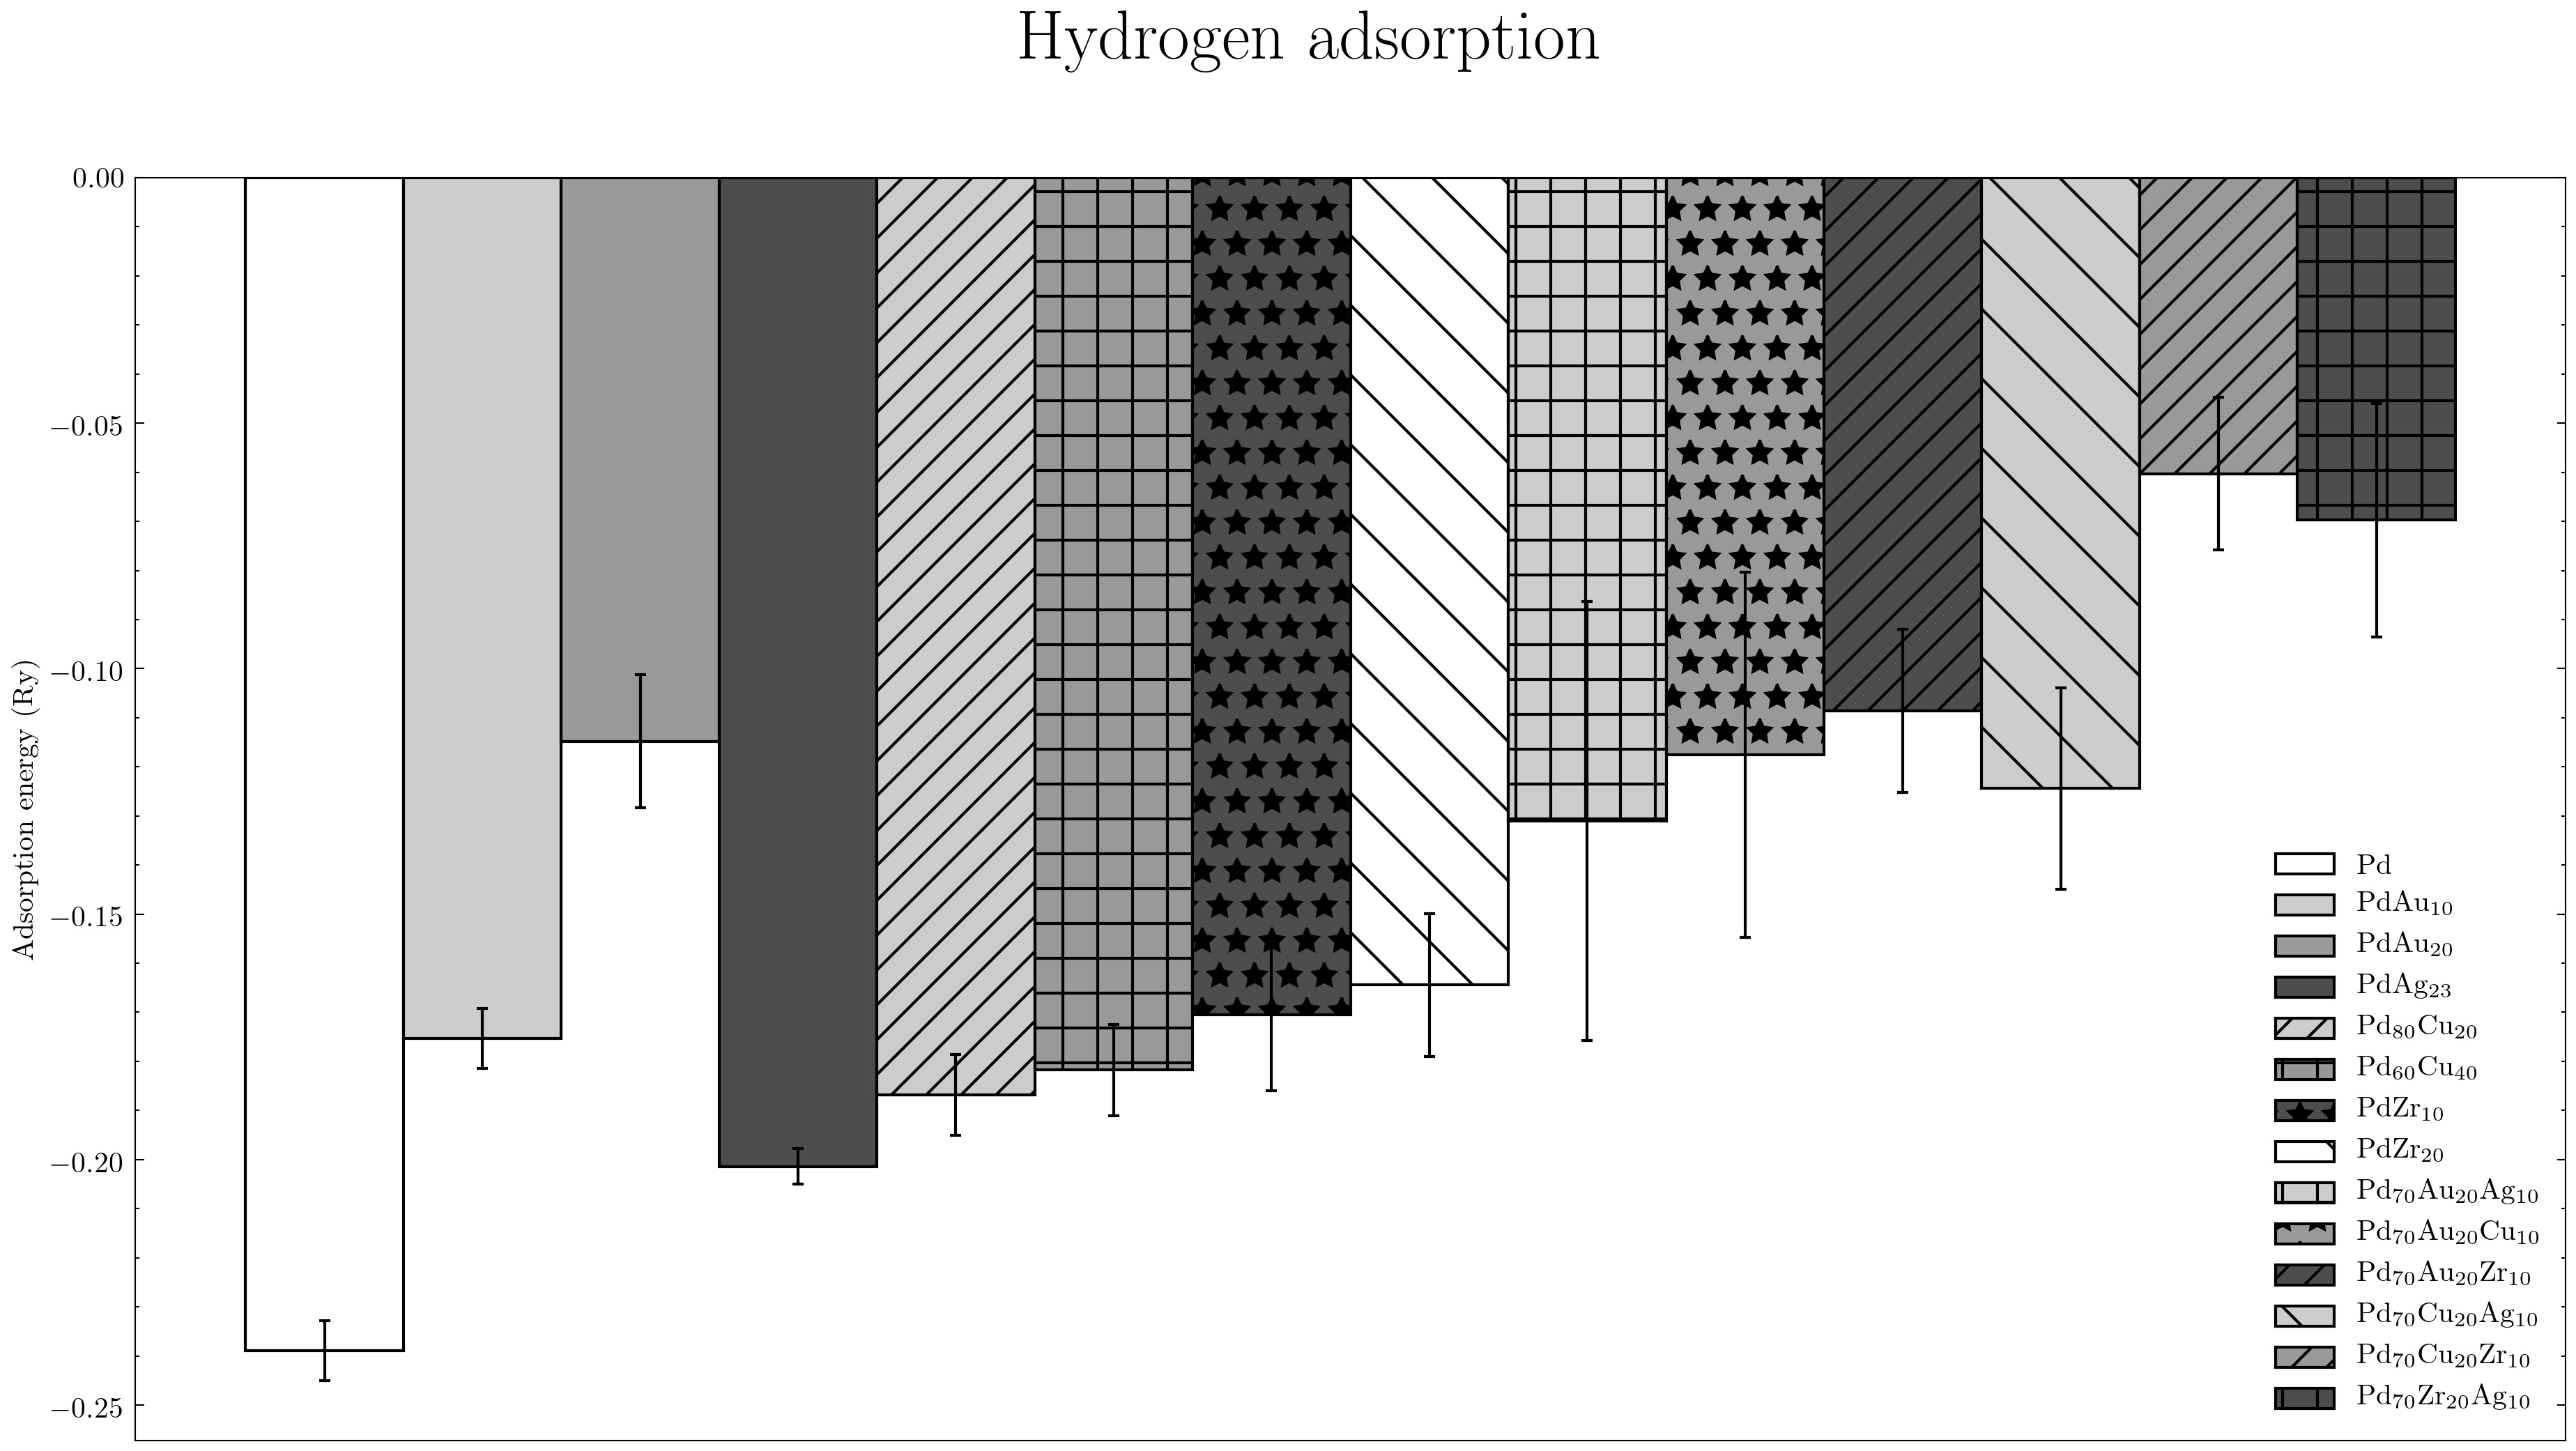
\includegraphics[width=0.9\linewidth,height=\textheight, keepaspectratio]{/Users/marc/Thesis/Chapter3/data/h2ads.jpg}
    \caption{Average adsorption energy of H\textsubscript{2} on the surface of palladium and palladium alloy slabs}
    \label{h2ads}
  \end{figure}

\end{landscape}
\subsubsection{Helium, Nitrogen, Carbon Dioxide and Argon}
\begin{landscape}
    \begin{figure}
        \centering
        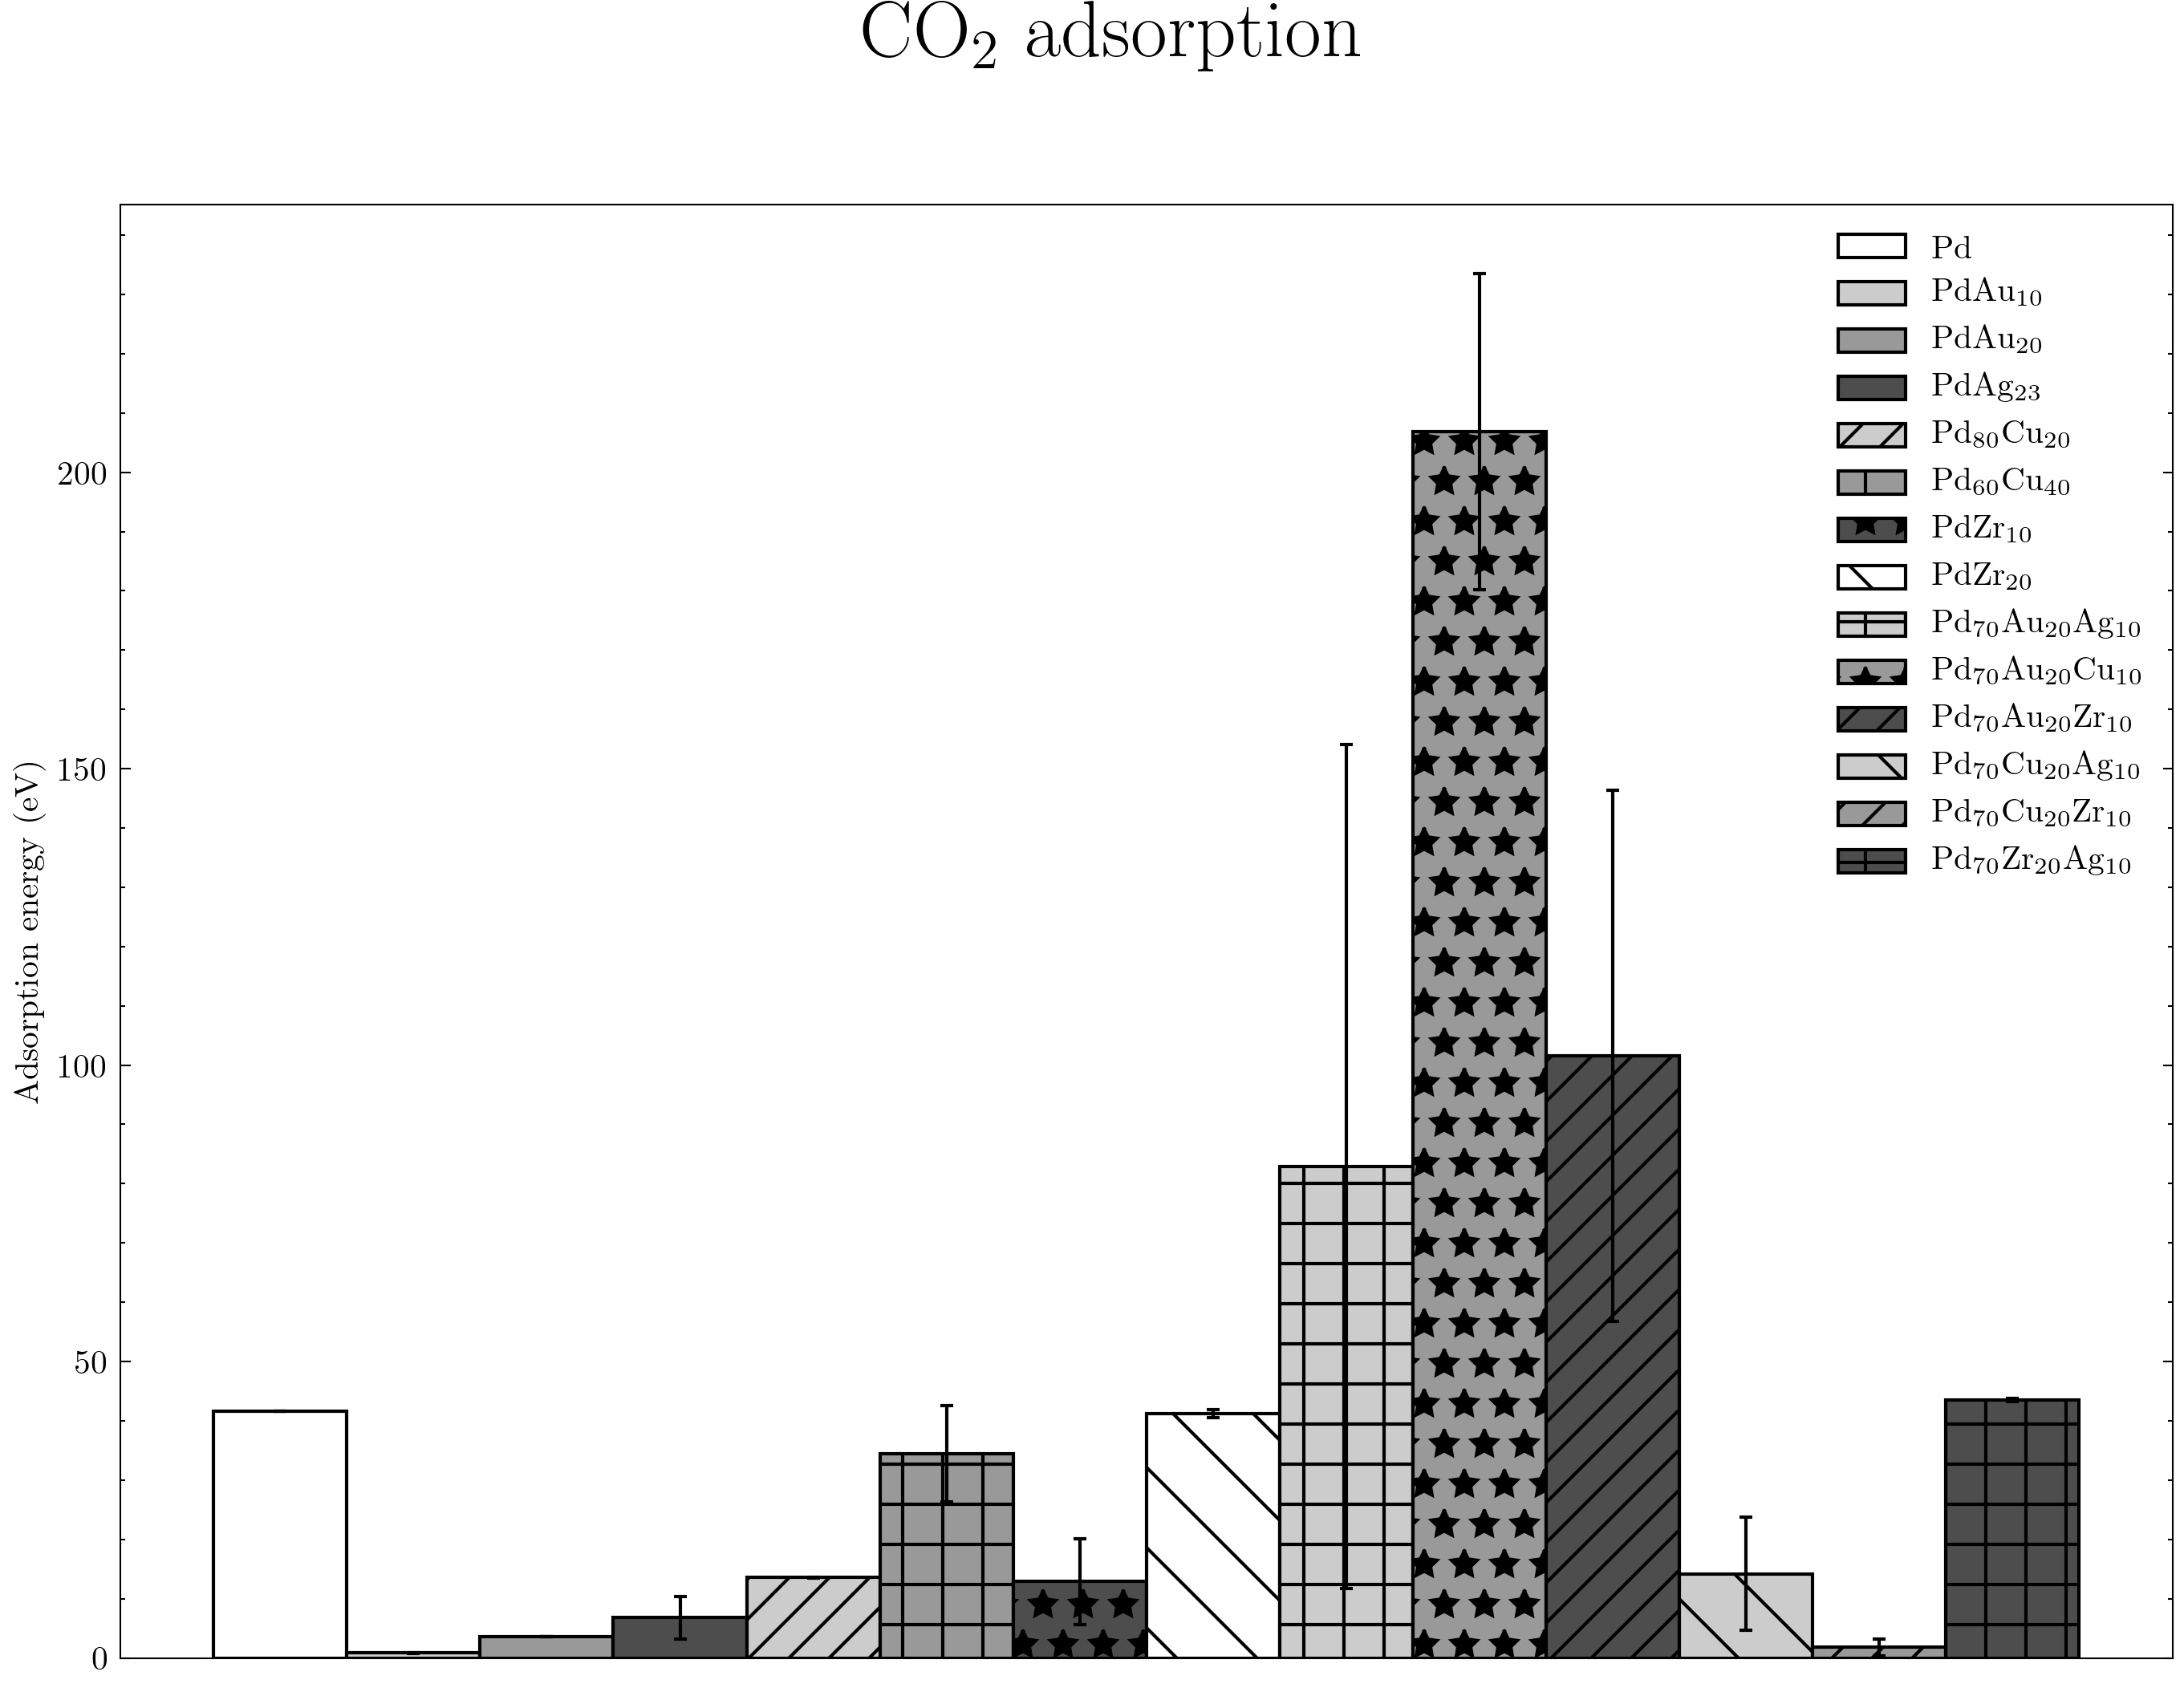
\includegraphics[width=0.9\linewidth,height=\textheight, keepaspectratio]{/Users/marc/Thesis/Chapter3/data/CO2ads.jpg}
        \caption{Average adsorption energy of CO\textsubscript{2} on the surface of palladium and palladium alloy slabs}
        \label{h2ads}
      \end{figure}
    
    \end{landscape}

    \begin{landscape}
        \begin{figure}
            \centering
            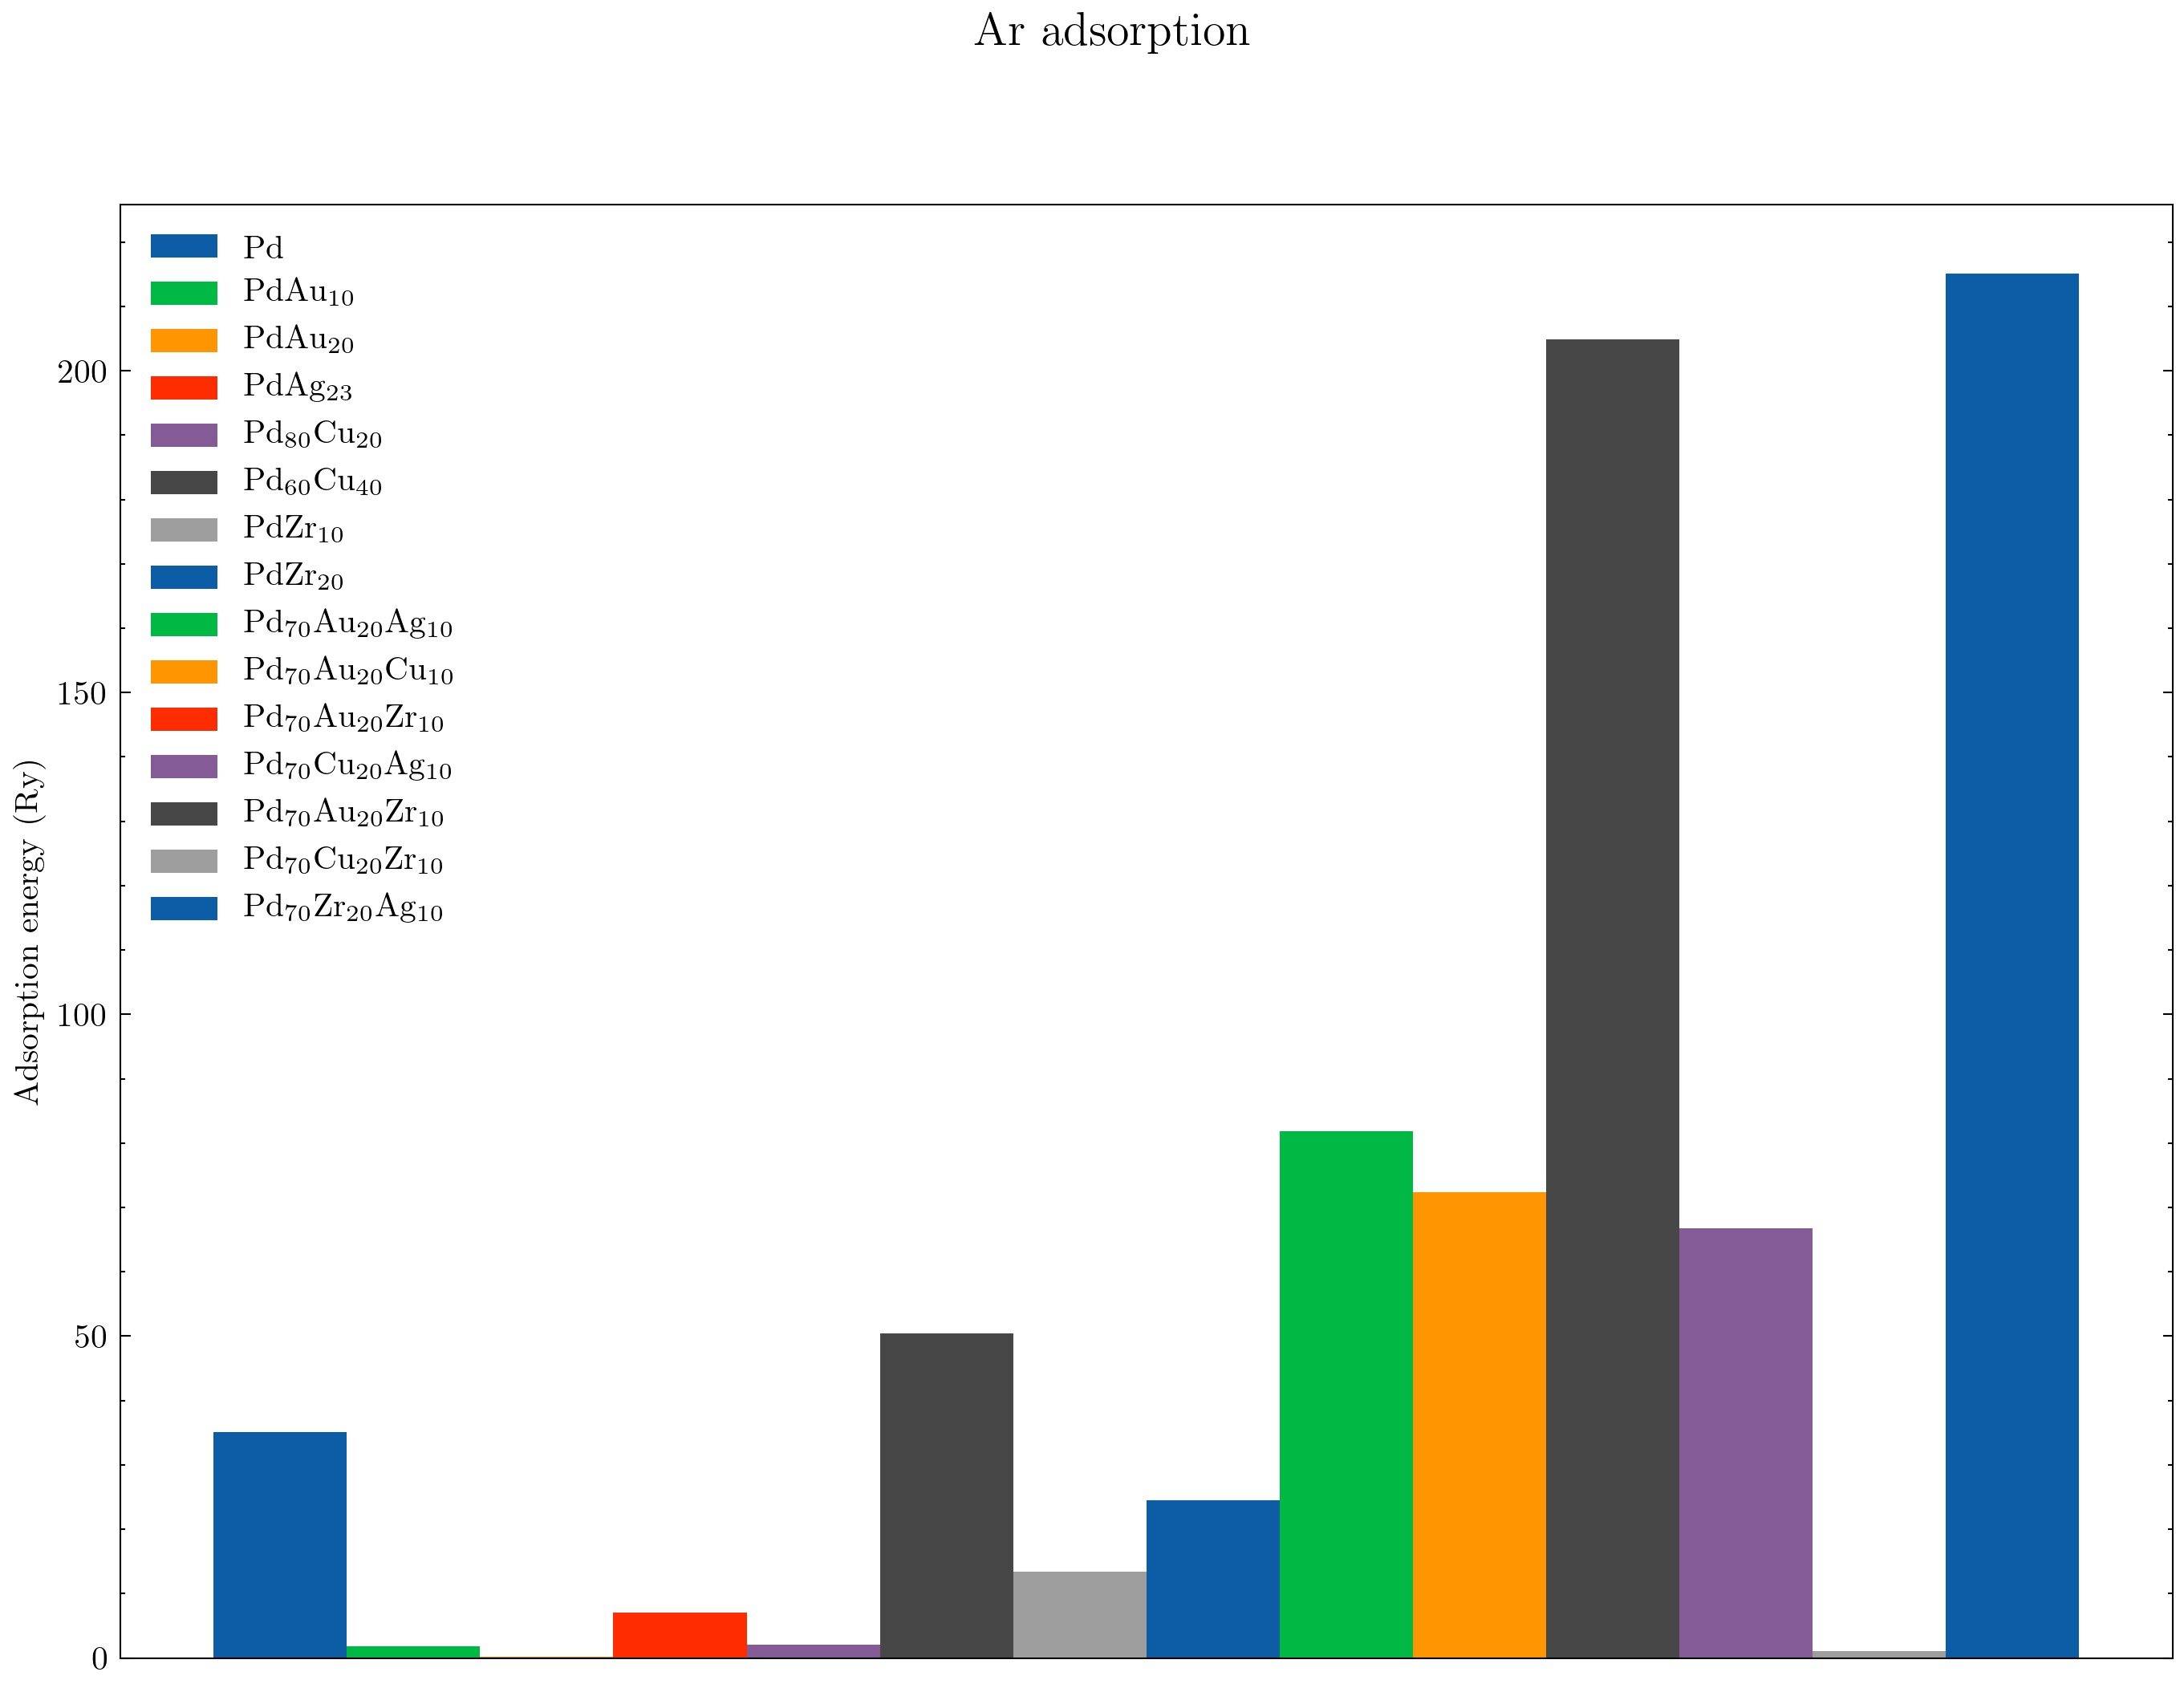
\includegraphics[width=0.9\linewidth,height=\textheight, keepaspectratio]{/Users/marc/Thesis/Chapter3/data/ARads.jpg}
            \caption{Average adsorption energy of Ar on the surface of palladium and palladium alloy slabs}
            \label{h2ads}
          \end{figure}
        
        \end{landscape}
\subsubsection{Carbon Monoxide}

\begin{landscape}
    \begin{figure}
        \centering
        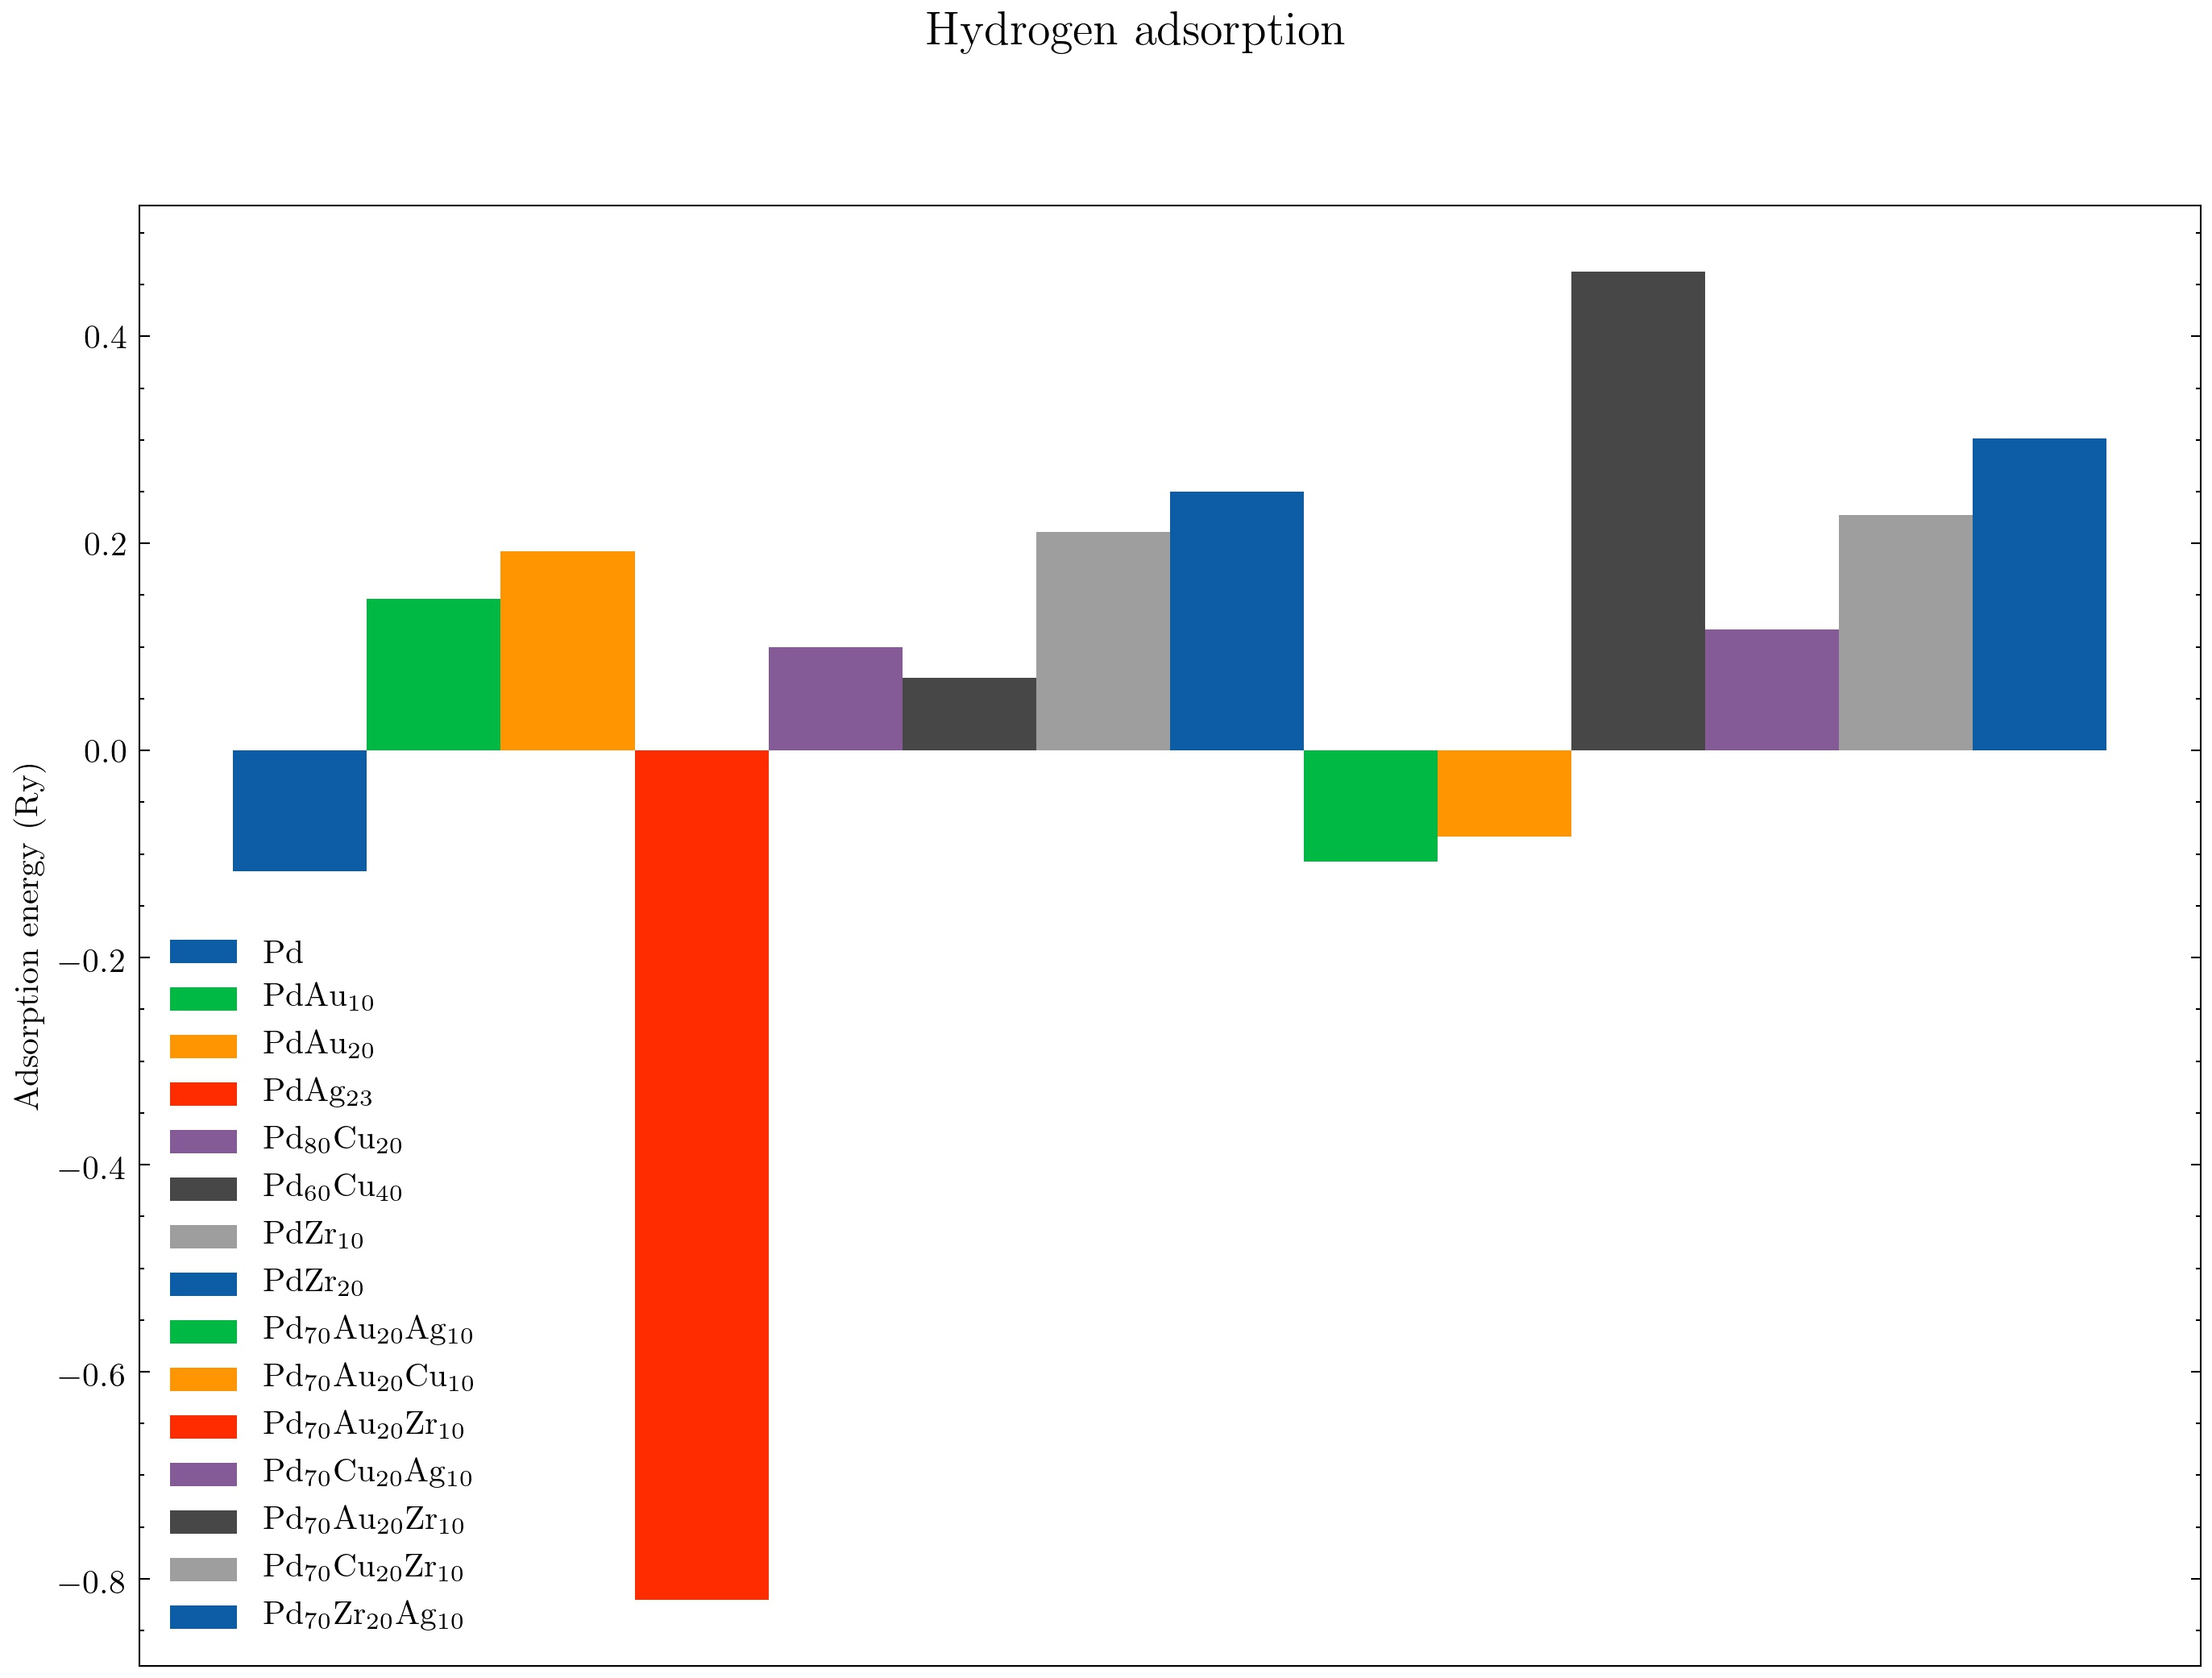
\includegraphics[width=0.9\linewidth,height=\textheight, keepaspectratio]{/Users/marc/Thesis/Chapter3/data/COads.jpg}
        \caption{Average adsorption energy of CO on the surface of palladium and palladium alloy slabs}
        \label{h2ads}
      \end{figure}
    
    \end{landscape}
\subsubsection{Carbon Dioxide}
\subsubsection{Ammonia}
\subsubsection{Oxygen}
\subsubsection{Water}
\subsubsection{Methane}
\subsubsection{Formaldehyde}
\subsubsection{Formic Acid}
\subsubsection{Hydrogen sulphide}
\begin{landscape}

\begin{figure}
    \centering
    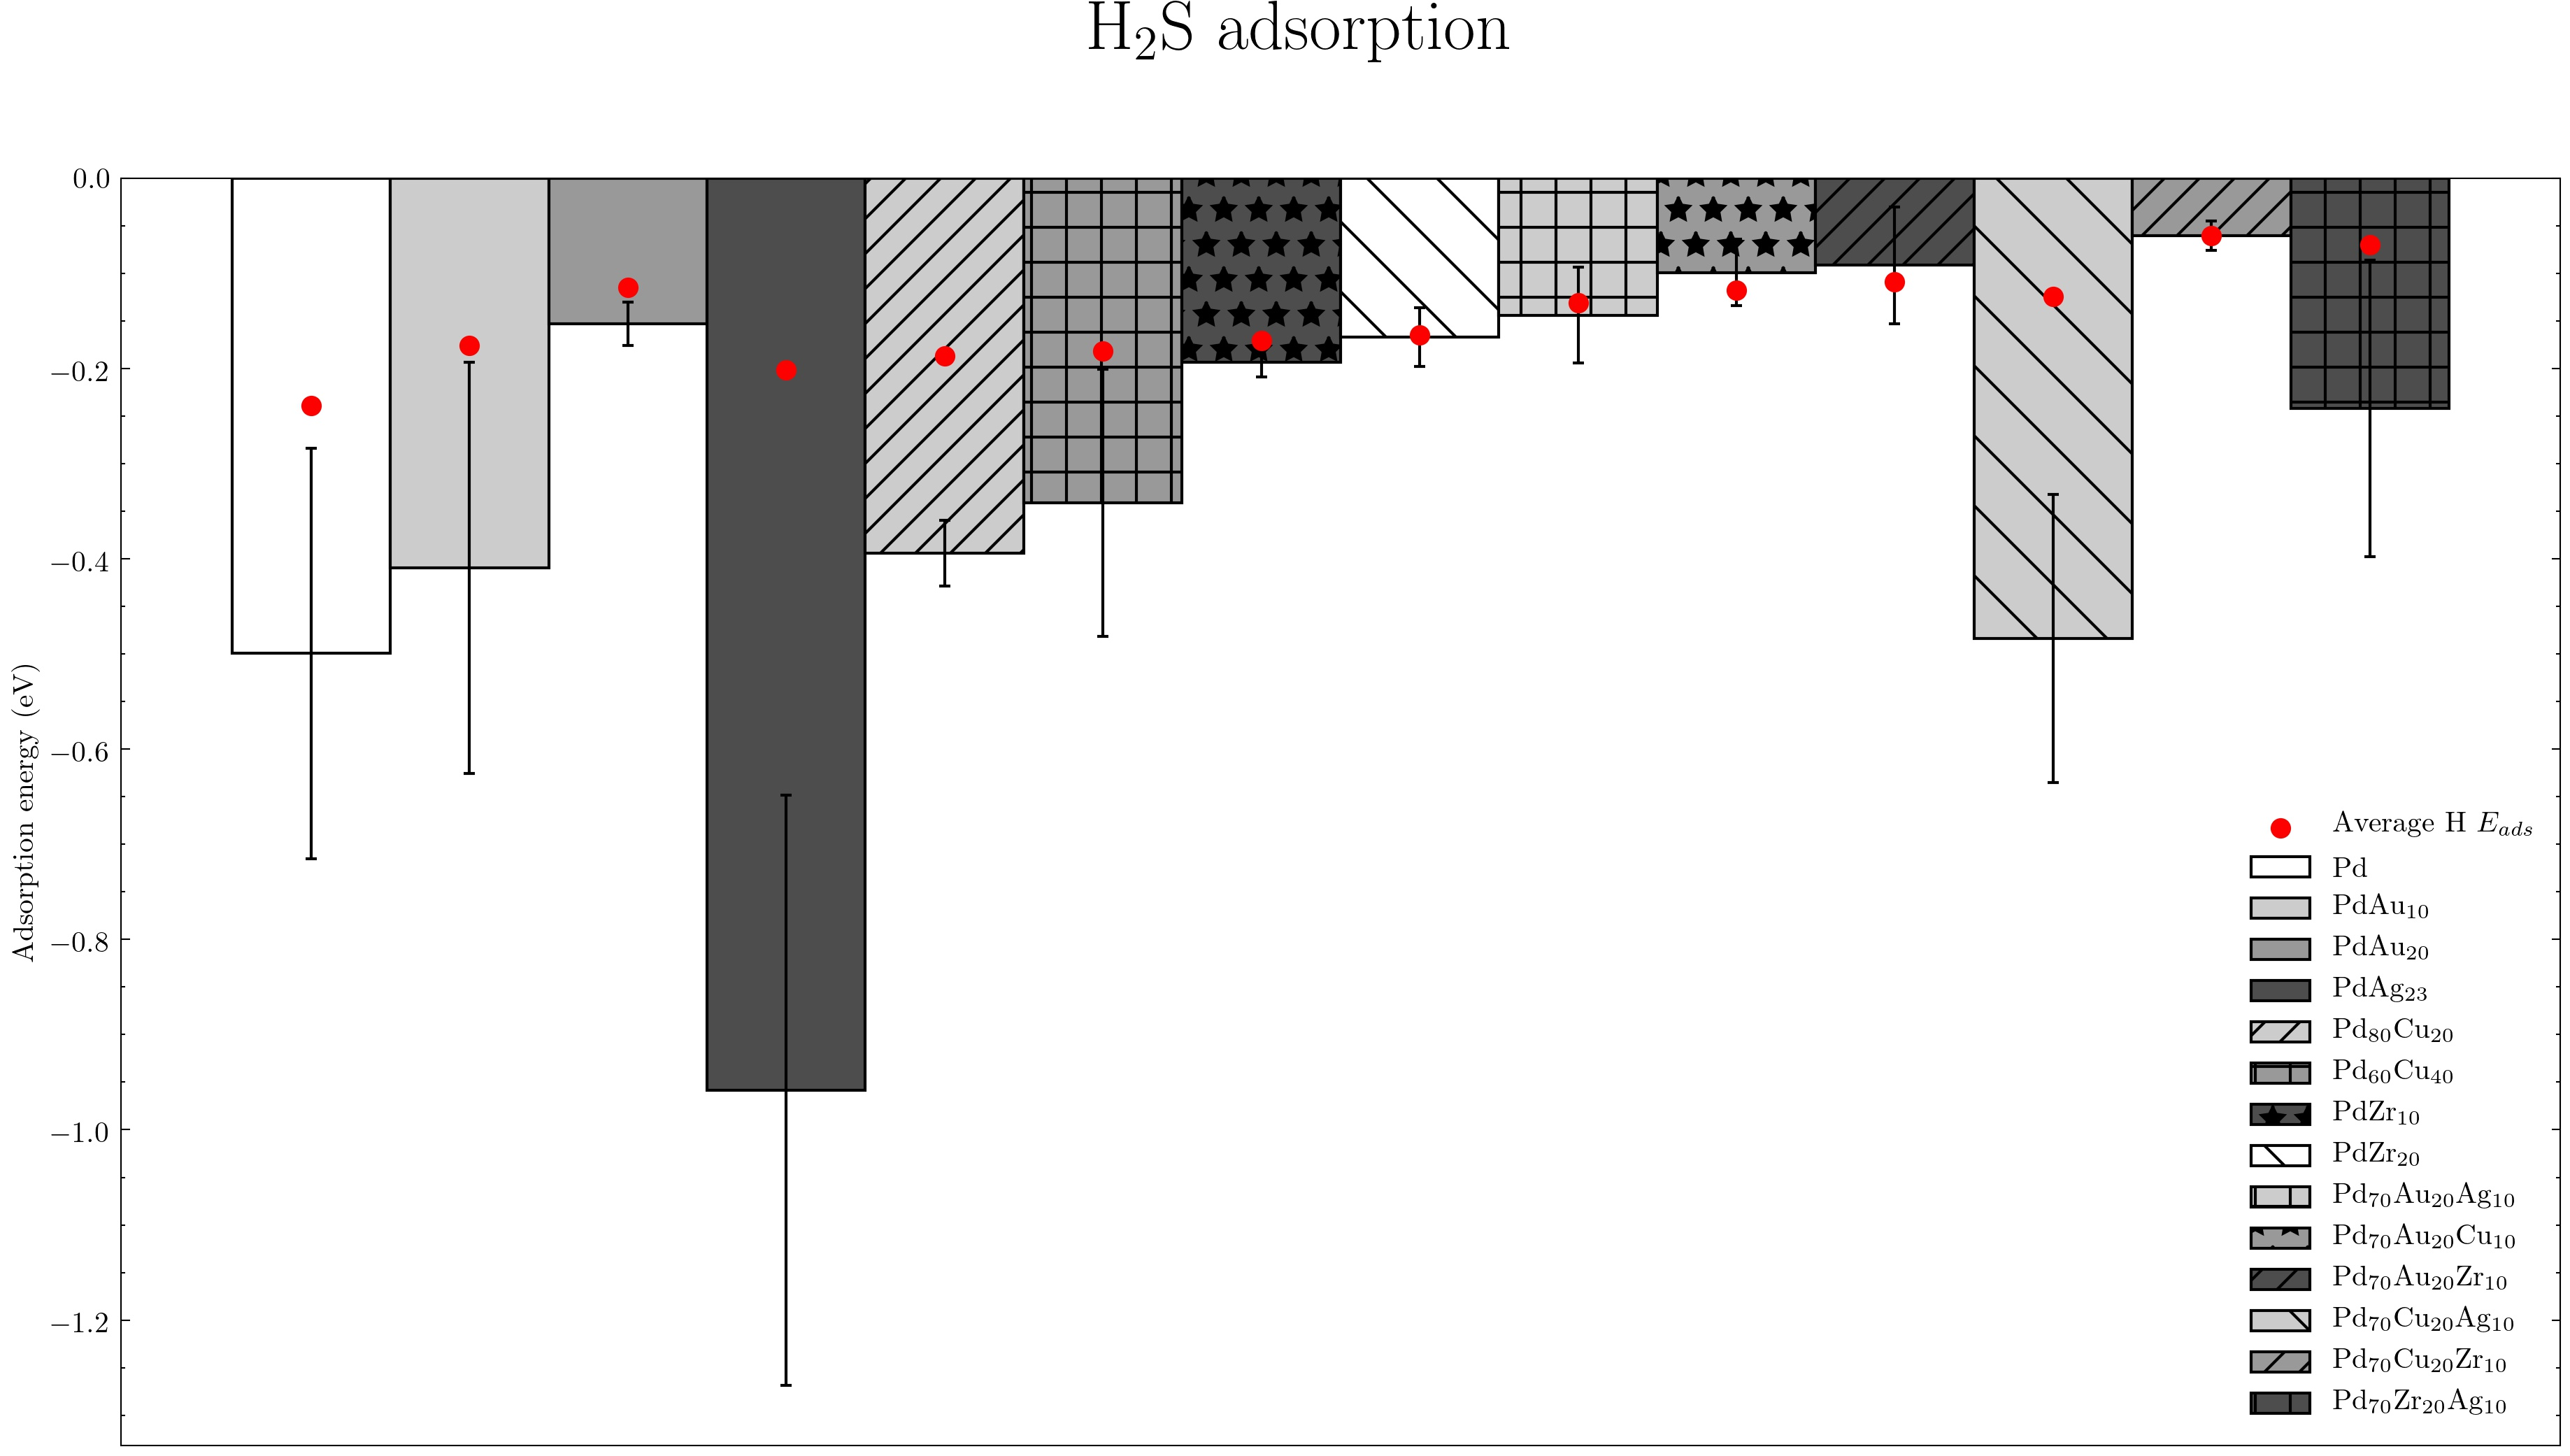
\includegraphics[width=0.9\linewidth,height=\textheight, keepaspectratio]{/Users/marc/Thesis/Chapter3/data/H2Sads.jpg}
    \caption{Average adsorption energy of H\textsubscript{2}S on the surface of palladium and palladium alloy slabs}
    \label{h2ads}
  \end{figure}
\end{landscape}


\section{Conclusion}
\bibliographystyle{plainnat}
\bibliography{library.bib}